
\section{Work done so far}

Work done so far in the task of Natural Language Inference can be divided as -

\begin{enumerate}
	\item Dataset Exploration
	\item Basic EDA and data pre-processing of selected dataset
	\item Experiments by fitting some basic ML/Language Modelling techniques.
\end{enumerate}


\subsection{Dataset Exploration}
As described above, we have explored 2 datasets i.e., SNLI and MultiNLI datasets for NLI tasks. We will be continuing with the SNLI dataset as for SNLI the test dataset is  available which is not the case with MultiNLI.

\subsection{Basic EDA and Data Pre-processing}
Basic EDA and data pre-processing has been done on SNLI dataset. This includes – 
\begin{enumerate}
	\item Identified the columns that contained only NULL values and removed them.
	\item Visualized the distribution of each gold label (Contradiction, Neutral, Entailment) using histogram and removed any samples that contained irrelevant label(s).
\end{enumerate}

\begin{figure}[h]
	\centering
	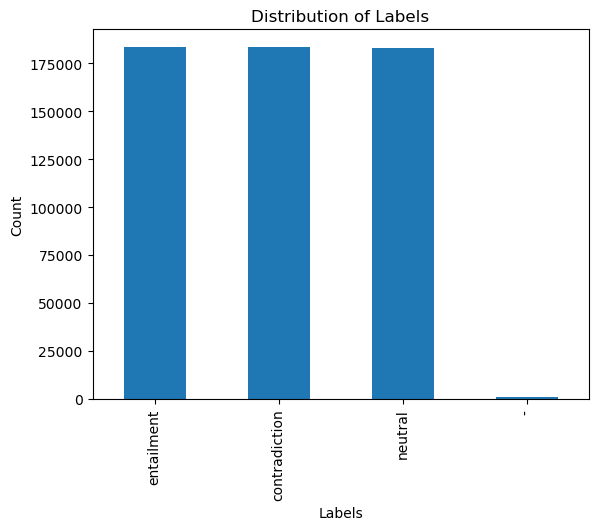
\includegraphics[scale=0.7]{img/label_distribution.png}
	\caption{Label Distribution of the SNLI Dataset}
\end{figure}

\begin{itemize}
	\item Identified any NULL premises or hypothesis and removed them from the dataset.
	\item Converted all premise and hypothesis to lowercase to ensure consistency in the dataset.
	\item Analysed the statistical parameters of premise and hypothesis that helped to better understand SNLI dataset.
	\item Encoded the gold labels to numerical categories.
	\item Identified the most frequently occurring 20 words in premise sentences.
\end{itemize}

\begin{figure}[h]
	\centering
	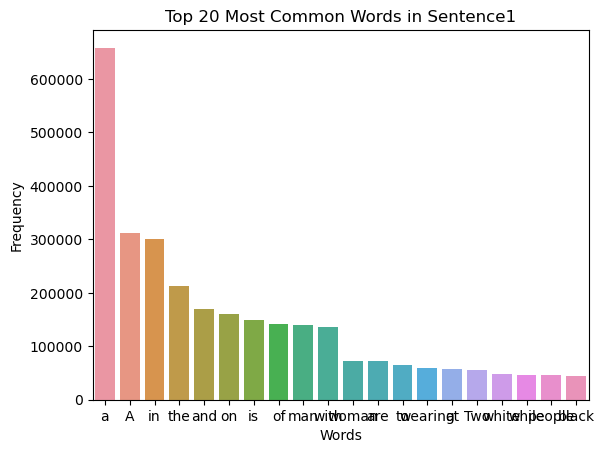
\includegraphics[scale=0.9]{img/word_dist.png}
	\caption{Word Distribution in \texttt{sentence1}}
\end{figure}


\subsection{Experiments with ML/Language Modelling techniques}

Experiments have been performed by fitting some ML /Language Modelling Techniques and finding the accuracy in each of the applied methods.

\subsubsection{Logistic Regression}
To perform logistic regression on a dataset containing premises and hypotheses, the premises and hypotheses are first concatenated. The concatenated data is then transformed using TfidfVectorizer, which includes stop word removal. The resulting data is used to fit a logistic regression model with \textit{\textbf{max\_iter = 10000}}.

The trained logistic regression model is then used to predict the premises and hypotheses of a separate test dataset. The premises and hypotheses of the test dataset are transformed using the same TfidfVectorizer used during training before being fed into the logistic regression model for prediction.

Classification report and accuracy score is calculated over test data as shown below

\begin{figure}[h]
	\centering
	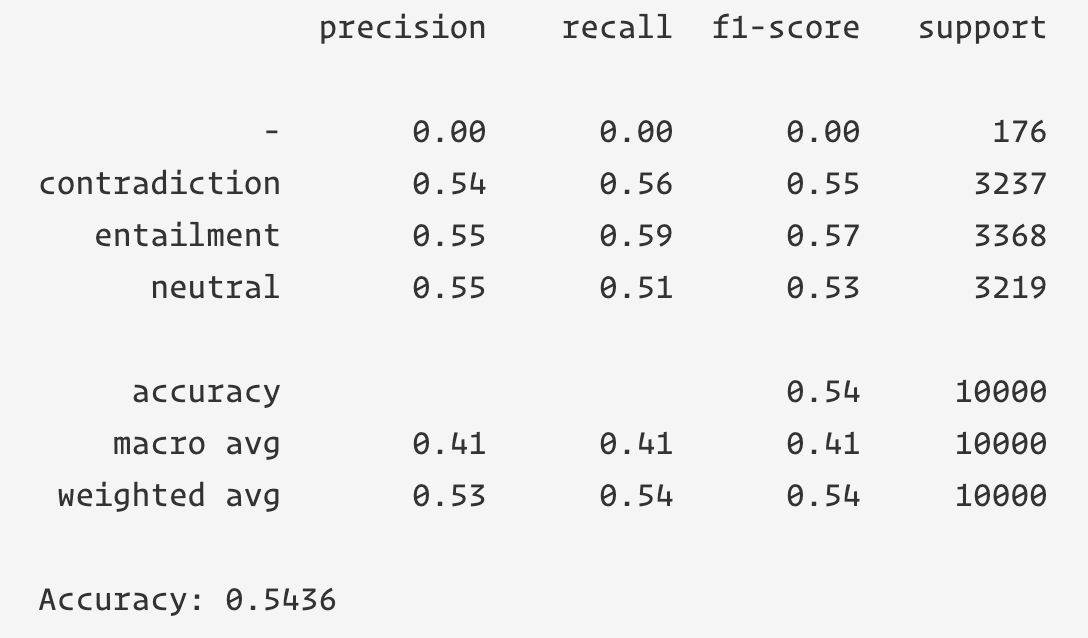
\includegraphics[scale=0.7]{img/logicf1.png}
	\caption{F1 Score using Logistic Regression}
\end{figure}

\textit{\textbf{Accuracy on Test Data on applying Logistic regression is 54.36\%.}}


\subsubsection{Logistic Regression with Hyperparameter Tuning}

We will be continuing with train and test data obtained after processing from TfidfVectorizer, implemented in the Logistic Regression model above. 

\textit{\textbf{GridSearchCV}}\cite{gdsearch} is used to tune the hyperparameter and then predict the test data on the best hyperparameters found using grid search.


\begin{lstlisting}[language=Python]
# Hyperparameter tuning
param_grid = {'C': [0.1, 1, 10]}
grid_search = GridSearchCV(lr, param_grid, cv=5, verbose=2, n_jobs=-1)
grid_search.fit(X_train, label_list)

y_pred = grid_search.predict(X_test)
\end{lstlisting}


The hyperparameter that is being tuned here is the regularization parameter \textit{\textbf{'C'}} with 3 different values: [0.1, 1, 10].

For hyperparameter tuning, here we have used the \textit{\textbf{GridSearchCV}} from scikit learn library.  The parameter \textit{\textbf{'cv'}} specifies the number of cross validation folds, \textit{\textbf{'n\_jobs'}} specifies the number of CPU cores to be used in parallel, and \textit{\textbf{'verbose'}} controls the output that will be printed on screen.

The fit method on grid\_search object is called on train data and labels to train a Logistic regression model with different hyperparameters using cross validation. The \textit{\textbf{'predict'}} method on test data using the best hyperparameters found during gris search.

Classification report and accuracy score is calculated over test data as shown below

\begin{figure}[h]
	\centering
	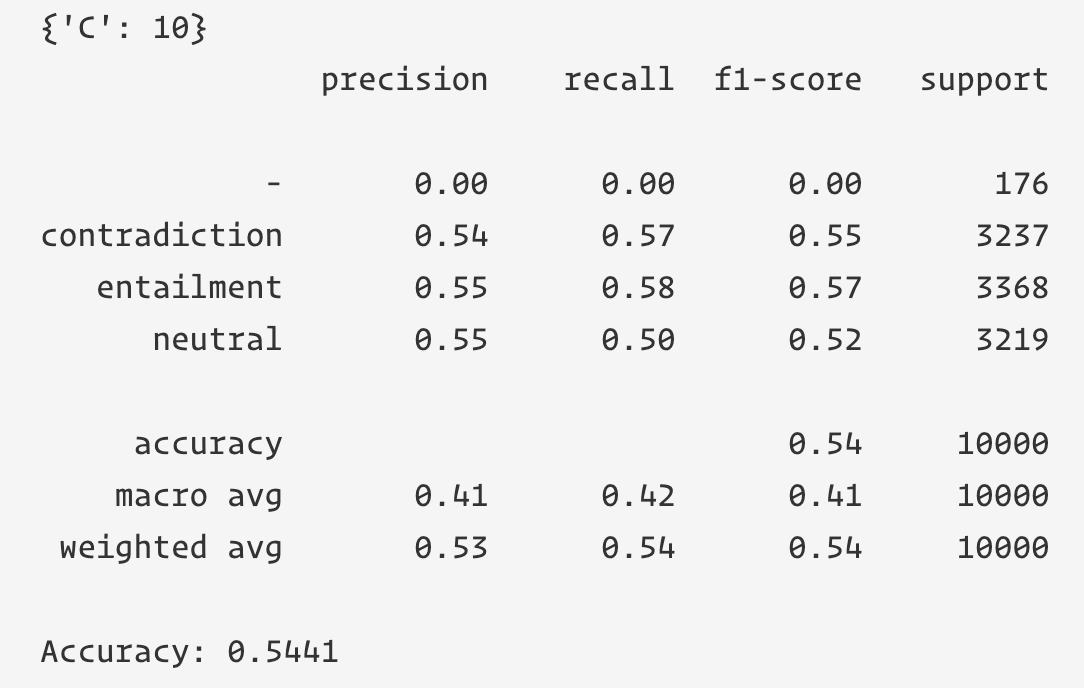
\includegraphics[scale=0.7]{img/hyperlogicf1.png}
	\caption{F1 Score using Logistic Regression and Hyper-parameter tuning}
\end{figure}

\textit{\textbf{Out of the provided 3 values for regularization factor C; the best it can do is at C = 10 and generates an accuracy of 54.41\%.}}


\subsubsection{Bi-directional LSTM}

To perform the Natural Language Inference task, a Bidirectional LSTM model is utilized. For this, the very first step is to use \textit{\textbf{nltk Tokenizer}} maximum vocabulary size as 5000 and out of vocabulary word as \textit{\textbf{"OOV"}}.  Concatenated train premise and hypothesis are then processed to generate word indices from the nltk tokenizer.  The generated word indices are used to convert each sentence (concatenated premise and hypothesis) of train, validation and test to their equivalent numerical vector representation.

Before fitting the Neural Language Model, each sentence is padded with zeroes to make each sentence of equal length. Label lists for validation and test data are converted into their equivalent one-hot vector representation prior to being passed to the layers of NLM.

Here we have used \textit{\textbf{Keras}} deep learning framework.

The layers that are added to build the NLM for NLI task are -

\begin{figure}
	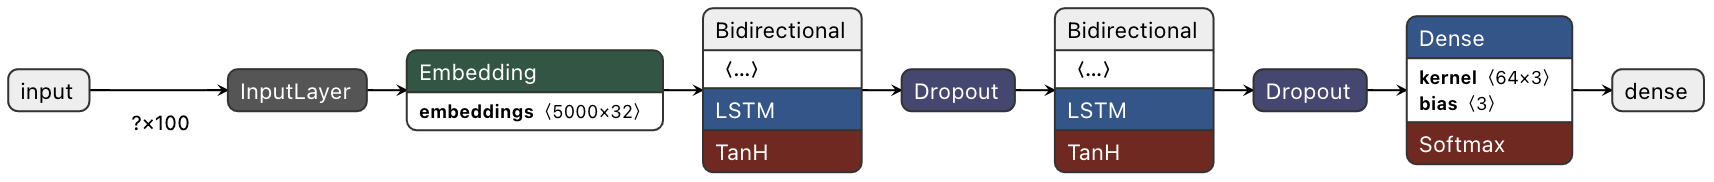
\includegraphics[scale=0.3]{img/model_image_comp.png}
	\caption{BiLSTM Model Visualisation}
\end{figure}

\begin{itemize}
	\item The first layer is an Embedding layer that takes the sentences where each sentence is of size max\_len (== 100) and converts each word into a dense vector representation of size 32 (embedding dimension).
	\item The output from Embedding layer is then forwarded to Bidirectional LSTM layer with hidden dimension size 64.
	\item The third layer is a dropout layer. Dropout is a regularization technique that randomly drops out a proportion of the units (here 50\%) in the layer during training and helps to prevent overfitting.
	\item The fourth layer is another bidirectional LSTM layer, with  32 units as hidden dimension.
	\item The fifth layer is another dropout layer, which helps to prevent overfitting.
	\item The final layer is a dense layer with num\_classes units and a softmax activation function. The num\_classes parameter specifies the number of classes in the classification problem, (here num\_classes = 3) and the softmax activation function outputs the predicted class probabilities.
	\item The class for which probability is maximum will be selected as the label for premise-hypothesis pair.
\end{itemize}

The optimizer used is Adam Optimizer along with the Categorical Cross Entropy loss function with accuracy metric. The goal is to minimize the categorical cross-entropy loss and maximize the accuracy metric.

\begin{lstlisting}[language=Python]
model.compile(optimizer='adam', loss='categorical_crossentropy', metrics=['accuracy'], run_eagerly=True)
\end{lstlisting}

The model is trained with applied checkpoints that will save the best model based on validation data accuracy. Also early stopping criteria is applied to prevent overfitting. The batch size taken for training the model is 128.


\begin{lstlisting}[language=Python]

# Train the model
es = EarlyStopping(monitor='val_loss', mode='min', verbose=1, patience=3)
mc = ModelCheckpoint('best_model.h5', monitor='val_accuracy', mode='max', verbose=1, save_best_only=True)


history = model.fit(X_train, y_train, validation_data=(X_val, y_val), epochs=20, batch_size=128, callbacks=[mc, es])


\end{lstlisting}


The labels for test premise and hypothesis pair are predicted using the best saved model.

Classification report and accuracy score is calculated over test data as shown below-
\pagebreak

\begin{figure}[h]
	\centering
	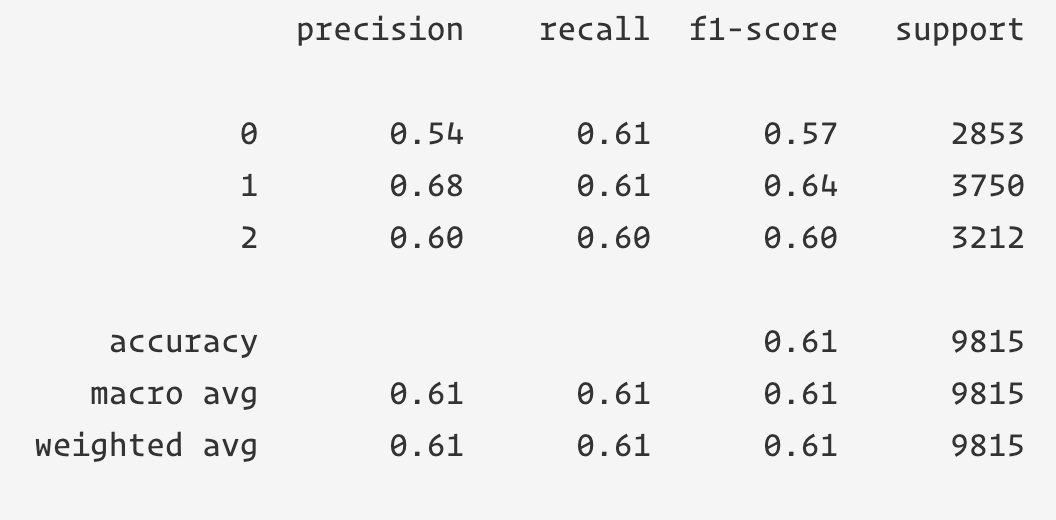
\includegraphics[scale=0.7]{img/bilstmf1.png}
	\caption{F1 Score using BiLSTM}
\end{figure}


\section{Conclusion of work done so far}
Three models were evaluated for the Natural Language Inference task, which involves determining whether a given sentence (hypothesis) can be inferred from another sentence (premise) or not. The models included Logistic Regression, Logistic Regression with hyperparameter tuning, and Bi-directional LSTM. The Results are as follows - 

\begin{itemize}
	\item Accuracy with Logistic Regression comes out to be – \textit{\textbf{54.36\%}}
	\item Accuracy with Logistic Regression with hyperparameter tuning comes out to be – \textit{\textbf{54.41\%}}
	\item Accuracy with Bi-directional LSTM comes out to be – \textit{\textbf{61\%}}

\end{itemize}

















